%% bare_conf.tex
%% V1.4b
%% 2015/08/26
%% by Michael Shell
%% See:
%% http://www.michaelshell.org/
%% for current contact information.
%%
%% This is a skeleton file demonstrating the use of IEEEtran.cls
%% (requires IEEEtran.cls version 1.8b or later) with an IEEE
%% conference paper.
%%
%% Support sites:
%% http://www.michaelshell.org/tex/ieeetran/
%% http://www.ctan.org/pkg/ieeetran
%% and
%% http://www.ieee.org/

%%*************************************************************************
%% Legal Notice:
%% This code is offered as-is without any warranty either expressed or
%% implied; without even the implied warranty of MERCHANTABILITY or
%% FITNESS FOR A PARTICULAR PURPOSE! 
%% User assumes all risk.
%% In no event shall the IEEE or any contributor to this code be liable for
%% any damages or losses, including, but not limited to, incidental,
%% consequential, or any other damages, resulting from the use or misuse
%% of any information contained here.
%%
%% All comments are the opinions of their respective authors and are not
%% necessarily endorsed by the IEEE.
%%
%% This work is distributed under the LaTeX Project Public License (LPPL)
%% ( http://www.latex-project.org/ ) version 1.3, and may be freely used,
%% distributed and modified. A copy of the LPPL, version 1.3, is included
%% in the base LaTeX documentation of all distributions of LaTeX released
%% 2003/12/01 or later.
%% Retain all contribution notices and credits.
%% ** Modified files should be clearly indicated as such, including  **
%% ** renaming them and changing author support contact information. **
%%*************************************************************************


% *** Authors should verify (and, if needed, correct) their LaTeX system  ***
% *** with the testflow diagnostic prior to trusting their LaTeX platform ***
% *** with production work. The IEEE's font choices and paper sizes can   ***
% *** trigger bugs that do not appear when using other class files.       ***                          ***
% The testflow support page is at:
% http://www.michaelshell.org/tex/testflow/



\documentclass[conference]{IEEEtran}
% Some Computer Society conferences also require the compsoc mode option,
% but others use the standard conference format.
%
% If IEEEtran.cls has not been installed into the LaTeX system files,
% manually specify the path to it like:
% \documentclass[conference]{../sty/IEEEtran}





% Some very useful LaTeX packages include:
% (uncomment the ones you want to load)


% *** MISC UTILITY PACKAGES ***
%
%\usepackage{ifpdf}
% Heiko Oberdiek's ifpdf.sty is very useful if you need conditional
% compilation based on whether the output is pdf or dvi.
% usage:
% \ifpdf
%   % pdf code
% \else
%   % dvi code
% \fi
% The latest version of ifpdf.sty can be obtained from:
% http://www.ctan.org/pkg/ifpdf
% Also, note that IEEEtran.cls V1.7 and later provides a builtin
% \ifCLASSINFOpdf conditional that works the same way.
% When switching from latex to pdflatex and vice-versa, the compiler may
% have to be run twice to clear warning/error messages.






% *** CITATION PACKAGES ***
%
\usepackage{cite}
% cite.sty was written by Donald Arseneau
% V1.6 and later of IEEEtran pre-defines the format of the cite.sty package
% \cite{} output to follow that of the IEEE. Loading the cite package will
% result in citation numbers being automatically sorted and properly
% "compressed/ranged". e.g., [1], [9], [2], [7], [5], [6] without using
% cite.sty will become [1], [2], [5]--[7], [9] using cite.sty. cite.sty's
% \cite will automatically add leading space, if needed. Use cite.sty's
% noadjust option (cite.sty V3.8 and later) if you want to turn this off
% such as if a citation ever needs to be enclosed in parenthesis.
% cite.sty is already installed on most LaTeX systems. Be sure and use
% version 5.0 (2009-03-20) and later if using hyperref.sty.
% The latest version can be obtained at:
% http://www.ctan.org/pkg/cite
% The documentation is contained in the cite.sty file itself.






% *** GRAPHICS RELATED PACKAGES ***
%
\ifCLASSINFOpdf
  \usepackage[pdftex]{graphicx}
  % declare the path(s) where your graphic files are
  \graphicspath{ {images/} }
  % and their extensions so you won't have to specify these with
  % every instance of \includegraphics
  % \DeclareGraphicsExtensions{.pdf,.jpeg,.png}
\else
  % or other class option (dvipsone, dvipdf, if not using dvips). graphicx
  % will default to the driver specified in the system graphics.cfg if no
  % driver is specified.
  % \usepackage[dvips]{graphicx}
  % declare the path(s) where your graphic files are
  % \graphicspath{{../eps/}}
  % and their extensions so you won't have to specify these with
  % every instance of \includegraphics
  % \DeclareGraphicsExtensions{.eps}
\fi
% graphicx was written by David Carlisle and Sebastian Rahtz. It is
% required if you want graphics, photos, etc. graphicx.sty is already
% installed on most LaTeX systems. The latest version and documentation
% can be obtained at: 
% http://www.ctan.org/pkg/graphicx
% Another good source of documentation is "Using Imported Graphics in
% LaTeX2e" by Keith Reckdahl which can be found at:
% http://www.ctan.org/pkg/epslatex
%
% latex, and pdflatex in dvi mode, support graphics in encapsulated
% postscript (.eps) format. pdflatex in pdf mode supports graphics
% in .pdf, .jpeg, .png and .mps (metapost) formats. Users should ensure
% that all non-photo figures use a vector format (.eps, .pdf, .mps) and
% not a bitmapped formats (.jpeg, .png). The IEEE frowns on bitmapped formats
% which can result in "jaggedy"/blurry rendering of lines and letters as
% well as large increases in file sizes.
%
% You can find documentation about the pdfTeX application at:
% http://www.tug.org/applications/pdftex





% *** MATH PACKAGES ***
%
%\usepackage{amsmath}
% A popular package from the American Mathematical Society that provides
% many useful and powerful commands for dealing with mathematics.
%
% Note that the amsmath package sets \interdisplaylinepenalty to 10000
% thus preventing page breaks from occurring within multiline equations. Use:
%\interdisplaylinepenalty=2500
% after loading amsmath to restore such page breaks as IEEEtran.cls normally
% does. amsmath.sty is already installed on most LaTeX systems. The latest
% version and documentation can be obtained at:
% http://www.ctan.org/pkg/amsmath





% *** SPECIALIZED LIST PACKAGES ***
%
%\usepackage{algorithmic}
% algorithmic.sty was written by Peter Williams and Rogerio Brito.
% This package provides an algorithmic environment fo describing algorithms.
% You can use the algorithmic environment in-text or within a figure
% environment to provide for a floating algorithm. Do NOT use the algorithm
% floating environment provided by algorithm.sty (by the same authors) or
% algorithm2e.sty (by Christophe Fiorio) as the IEEE does not use dedicated
% algorithm float types and packages that provide these will not provide
% correct IEEE style captions. The latest version and documentation of
% algorithmic.sty can be obtained at:
% http://www.ctan.org/pkg/algorithms
% Also of interest may be the (relatively newer and more customizable)
% algorithmicx.sty package by Szasz Janos:
% http://www.ctan.org/pkg/algorithmicx




% *** ALIGNMENT PACKAGES ***
%
%\usepackage{array}
% Frank Mittelbach's and David Carlisle's array.sty patches and improves
% the standard LaTeX2e array and tabular environments to provide better
% appearance and additional user controls. As the default LaTeX2e table
% generation code is lacking to the point of almost being broken with
% respect to the quality of the end results, all users are strongly
% advised to use an enhanced (at the very least that provided by array.sty)
% set of table tools. array.sty is already installed on most systems. The
% latest version and documentation can be obtained at:
% http://www.ctan.org/pkg/array


% IEEEtran contains the IEEEeqnarray family of commands that can be used to
% generate multiline equations as well as matrices, tables, etc., of high
% quality.




% *** SUBFIGURE PACKAGES ***
%\ifCLASSOPTIONcompsoc
%  \usepackage[caption=false,font=normalsize,labelfont=sf,textfont=sf]{subfig}
%\else
%  \usepackage[caption=false,font=footnotesize]{subfig}
%\fi
% subfig.sty, written by Steven Douglas Cochran, is the modern replacement
% for subfigure.sty, the latter of which is no longer maintained and is
% incompatible with some LaTeX packages including fixltx2e. However,
% subfig.sty requires and automatically loads Axel Sommerfeldt's caption.sty
% which will override IEEEtran.cls' handling of captions and this will result
% in non-IEEE style figure/table captions. To prevent this problem, be sure
% and invoke subfig.sty's "caption=false" package option (available since
% subfig.sty version 1.3, 2005/06/28) as this is will preserve IEEEtran.cls
% handling of captions.
% Note that the Computer Society format requires a larger sans serif font
% than the serif footnote size font used in traditional IEEE formatting
% and thus the need to invoke different subfig.sty package options depending
% on whether compsoc mode has been enabled.
%
% The latest version and documentation of subfig.sty can be obtained at:
% http://www.ctan.org/pkg/subfig




% *** FLOAT PACKAGES ***
%
%\usepackage{fixltx2e}
% fixltx2e, the successor to the earlier fix2col.sty, was written by
% Frank Mittelbach and David Carlisle. This package corrects a few problems
% in the LaTeX2e kernel, the most notable of which is that in current
% LaTeX2e releases, the ordering of single and double column floats is not
% guaranteed to be preserved. Thus, an unpatched LaTeX2e can allow a
% single column figure to be placed prior to an earlier double column
% figure.
% Be aware that LaTeX2e kernels dated 2015 and later have fixltx2e.sty's
% corrections already built into the system in which case a warning will
% be issued if an attempt is made to load fixltx2e.sty as it is no longer
% needed.
% The latest version and documentation can be found at:
% http://www.ctan.org/pkg/fixltx2e


%\usepackage{stfloats}
% stfloats.sty was written by Sigitas Tolusis. This package gives LaTeX2e
% the ability to do double column floats at the bottom of the page as well
% as the top. (e.g., "\begin{figure*}[!b]" is not normally possible in
% LaTeX2e). It also provides a command:
%\fnbelowfloat
% to enable the placement of footnotes below bottom floats (the standard
% LaTeX2e kernel puts them above bottom floats). This is an invasive package
% which rewrites many portions of the LaTeX2e float routines. It may not work
% with other packages that modify the LaTeX2e float routines. The latest
% version and documentation can be obtained at:
% http://www.ctan.org/pkg/stfloats
% Do not use the stfloats baselinefloat ability as the IEEE does not allow
% \baselineskip to stretch. Authors submitting work to the IEEE should note
% that the IEEE rarely uses double column equations and that authors should try
% to avoid such use. Do not be tempted to use the cuted.sty or midfloat.sty
% packages (also by Sigitas Tolusis) as the IEEE does not format its papers in
% such ways.
% Do not attempt to use stfloats with fixltx2e as they are incompatible.
% Instead, use Morten Hogholm'a dblfloatfix which combines the features
% of both fixltx2e and stfloats:
%
% \usepackage{dblfloatfix}
% The latest version can be found at:
% http://www.ctan.org/pkg/dblfloatfix




% *** PDF, URL AND HYPERLINK PACKAGES ***
%
%\usepackage{url}
% url.sty was written by Donald Arseneau. It provides better support for
% handling and breaking URLs. url.sty is already installed on most LaTeX
% systems. The latest version and documentation can be obtained at:
% http://www.ctan.org/pkg/url
% Basically, \url{my_url_here}.




% *** Do not adjust lengths that control margins, column widths, etc. ***
% *** Do not use packages that alter fonts (such as pslatex).         ***
% There should be no need to do such things with IEEEtran.cls V1.6 and later.
% (Unless specifically asked to do so by the journal or conference you plan
% to submit to, of course. )

\usepackage{xspace}

% correct bad hyphenation here
\hyphenation{op-tical net-works semi-conduc-tor}

\newcommand{\so}{Stack Overflow\xspace}
\newcommand{\sitf}{{\sc StackInTheFlow}\xspace}

\begin{document}
%
% paper title
% Titles are generally capitalized except for words such as a, an, and, as,
% at, but, by, for, in, nor, of, on, or, the, to and up, which are usually
% not capitalized unless they are the first or last word of the title.
% Linebreaks \\ can be used within to get better formatting as desired.
% Do not put math or special symbols in the title.
\title{An Examination of the Parallelization of IR Metrics with Apache Spark \\ A Use Case}


% author names and affiliations
% use a multiple column layout for up to three different
% affiliations
\author{\IEEEauthorblockN{Chase Greco}
\IEEEauthorblockA{Virginia Commonwealth University \\
Richmond, Virginia, USA \\
grecocd@vcu.edu}}

% conference papers do not typically use \thanks and this command
% is locked out in conference mode. If really needed, such as for
% the acknowledgment of grants, issue a \IEEEoverridecommandlockouts
% after \documentclass

% for over three affiliations, or if they all won't fit within the width
% of the page, use this alternative format:
% 
%\author{\IEEEauthorblockN{Michael Shell\IEEEauthorrefmark{1},
%Homer Simpson\IEEEauthorrefmark{2},
%James Kirk\IEEEauthorrefmark{3}, 
%Montgomery Scott\IEEEauthorrefmark{3} and
%Eldon Tyrell\IEEEauthorrefmark{4}}
%\IEEEauthorblockA{\IEEEauthorrefmark{1}School of Electrical and Computer Engineering\\
%Georgia Institute of Technology,
%Atlanta, Georgia 30332--0250\\ Email: see http://www.michaelshell.org/contact.html}
%\IEEEauthorblockA{\IEEEauthorrefmark{2}Twentieth Century Fox, Springfield, USA\\
%Email: homer@thesimpsons.com}
%\IEEEauthorblockA{\IEEEauthorrefmark{3}Starfleet Academy, San Francisco, California 96678-2391\\
%Telephone: (800) 555--1212, Fax: (888) 555--1212}
%\IEEEauthorblockA{\IEEEauthorrefmark{4}Tyrell Inc., 123 Replicant Street, Los Angeles, California 90210--4321}}




% use for special paper notices
%\IEEEspecialpapernotice{(Invited Paper)}




% make the title area
\maketitle

% As a general rule, do not put math, special symbols or citations
% in the abstract
\begin{abstract}
The Apache Spark cluster-computing framework has the potential to drastically reduce the runtimes of tasks which are sufficiently parallelizable.  In this paper we present an examination of this capability through the use case of optimizing \sitf, a tool that generates interpretable queries to \so at the developer's behest.  Through our analysis, we observe that we can reduce the runtime of a step of the query generation process in half by leveraging Apache Spark.
\end{abstract}

% no keywords




% For peer review papers, you can put extra information on the cover
% page as needed:
% \ifCLASSOPTIONpeerreview
% \begin{center} \bfseries EDICS Category: 3-BBND \end{center}
% \fi
%
% For peerreview papers, this IEEEtran command inserts a page break and
% creates the second title. It will be ignored for other modes.
\IEEEpeerreviewmaketitle

\section{Introduction}
Software developers often consult the Web when searching for solutions to development issues they encounter.  The \so Q \& A forum, is one of the largest and most popular software development knowledgebases, with over 40 million monthly visitors, with an estimated 16.8 million professional developers and university students \cite{so_survey_2017}.

With such a large knowledgebase available, the potential exists for recommendation systems to increase developer productivity by managing and extracting those nuggets of information necessary to their task at hand.  Several recommendation tools aimed at \so have been proposed with this goal by integrating relevant information from \so directly into the IDE, such as Prompter \cite{ponzanelli2014mining} and SeaHawk \cite{ponzanelli2013seahawk} which automatically recommend posts from \so based on the context of the source code within the IDE.

In this paper we examine \sitf, a tool we have previously proposed which intends to automate the task of discovering relevant \so posts. \sitf is a personalized recommendation system which ties closely with developer behavior within the IDE, allowing them to remain in the flow of development.  It does this through several mechanisms, however, for the purposes of this paper we will focus on one such mechanism the \textbf{Auto Query} feature and examine the benefits parallelization via Apache Spark can provide it.

The structure of the remainder of this paper is as follows:
\begin{itemize}
	\item We present an overview of the Auto Query feature of \sitf, it's use case, and the procedure by which it generates queries
	\item We propose parallelization via Apache Spark as a method to speed up computation within the Auto Query generation process
	\item We examine the performance gains between our sequential and parallel implementations 
	\item We offer some conclusions as to the viability of this method
\end{itemize}

\section{Auto Query Generation}

\subsection{Use Case} \label{subsec:UseCase}
It may happen that when searching for the solution to a development problem the developer may not be able to form a query suitable to retrieve the information necessary to form a solution and may require assistance in query formulation.  For example, the developer may be seeking information on the configuration options for the \textit{SparkSession} object. In such a case she may highlight the section of code relevant to declaring or utilizing this object, right-click within the editor and select the \textit{Auto Query} option.  Utilizing a procedure detailed in Section \ref{subsec:QueryGen}, \sitf will then generate a query from the selected snippet which it then sends to the \so API to retrieve relevant results and display them within the IDE. From there she may browse the results, filter them by tags, or sort them by four different criteria: relevance, newest, last active, and number of votes.

\subsection{Query Generation Procedure} \label{subsec:QueryGen}
\sitf utilizes a four-step procedure for generating queries illustrated by Figure \ref{fig:overview}. In the first step, a dictionary is constructed offline from the posts contained within the \so Data Dump.  The data dump contains all user posts within the \so site and is published periodically by Stack Exchange. This dictionary is composed of terms extracted from the posts and for each term the \textit{collection term frequency}, \textit{document frequency}, \textit{inverse collection term frequency}, and \textit{inverse document frequency} are stored. Terms are selected from the body of posts based on the following criteria: They must begin with an upper or lowercase letter and they must be at least 2 characters in length. Upon storage in the dictionary, all terms are normalized to be lowercase.

\begin{figure*}[ht]
	\centering
	\caption{Overview of \sitf Query Generation.}
 	\label{fig:overview}
 	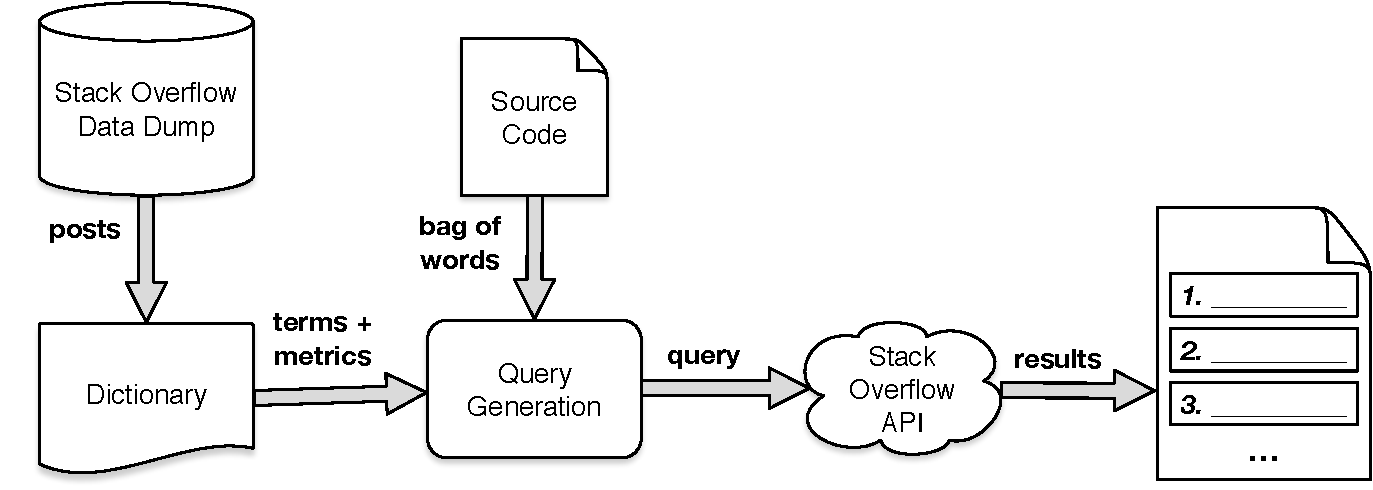
\includegraphics[width=.75\linewidth]{query-gen.pdf}
\end{figure*}

In the second step, when a snippet of code is received it is converted into a bag of words.  For each term within the bag of words, the corresponding metrics contained within the dictionary are examined. From these metrics several query pre-retrieval quality metrics such as \textit{tf-idf} are calculated and linearly summed to form an overall score for the term. Terms not contained within the dictionary are discarded. The top four scoring terms are then selected to form the candidate query.

In the third step, the candidate query is sent to the \so API to retrieval an initial results listing.

In the fourth step the results listing is retrieved as sent for additional processing before displaying it to the user.  If the candidate query returned no results and back-off technique is employed by incrementally removing lower scoring terms from the query.

\section{Apache Spark Parallelization}
The offline indexing of the \so Data Dump represents a significant commitment of computational resources to achieve, taking several hours to complete.  Though the computation is done offline and their is no direct impact to the user, it must be repeated each time a new data dump is released so that the model does not grow stale over time.  Due to the continued investment of resources necessary re-index future data dumps, efforts to parallelize this approach may be quite useful. Once more, the problem is further compounded by the ever-growing amount of posts contained within \so itself, meaning future data dumps will be even more resource-intensive to process.  In addition, decreasing the indexing run-time may allow for more sophisticated metrics to be computed and thereby enable a more complex recommendation model.

The current implementation of the indexer relies on a sequential parser.  The parser examines each post, one after the other, and keeps a running total of the \textit{collection term frequency} and \textit{document frequency} of the terms within the post. After processing all posts the \textit{inverse collection term frequency} and \textit{inverse document frequency} are calculated.

This approach, while effective, is a prime candidate for parallelization utilizing the \textit{MapReduce} paradigm of Apache Spark, as each post can be processed separately in parallel with the resultant calculations reduced to form the final metric calculations. We implement this approach in the following steps:
\begin{enumerate}
	\item For each post, map it's body into a bag of words, keeping track of the post from which they originate
	\item Filter each bag of words, performing term selection via the criteria previously described
	\item For each (post, term) paring, emit a one
	\item Perform a reduction on the term and compute a sum of each corresponding one to calculate \textit{Collection Term Frequency}
	\item Repeat the previous step for distinct (post, term) parings to calculate \textit{Document Frequency}
	\item From these metrics, calculate \textit{Inverse Collection Term Frequency} and \textit{Inverse Document Frequency}
\end{enumerate}

To examine this approach, we compare its runtime to that of the sequential parser for several sub-sets of the \so Data Dump of varying size. We ran our experiments on a cluster composed of 56 Intel Xeon E5-2690 CPUs clocked at 2.60GHz.

\section{Results}
The results of our analysis are given by Table \ref{tab:results}. 
\begin{table}[ht]
	\caption{Experimental Results}
	\label{tab:results}
	\begin{tabular}{|l|c|c|}
	\hline
	Number of Posts & Sequential Runtime (ms) & Spark Runtime (ms) \\
	\hline
	10 & \textbf{112} & 4865 \\
	100 & \textbf{158} & 4935 \\
	1000 & \textbf{308} & 6918 \\
	10000 & \textbf{1068} & 13161 \\
	100000 & \textbf{6587} & 28851 \\
	1000000 & 64722 & \textbf{44188} \\
	10000000 & 724983 & \textbf{354799} \\
	\hline
	\end{tabular}
\end{table}

We observe that for small datasets, the sequential parser soundly beats our Spark implementation. However, as the dataset size increases, the Spark implementation begins to overtake the sequential approach.  When examined graphically as in Figure \ref{fig:graph} we see that the sequential approach scales linearly with respect to the number of posts, which is to be expected. However, though the Spark implementation initially experiences a large jump in runtimes, it stables and begins to scale linearly with respect to the number of posts at a much slower rate, overtaking the sequential approach at about 60000 posts.

\begin{figure}[ht]
	\caption{Indexing Runtime vs Number of Posts}
	\label{fig:graph}
	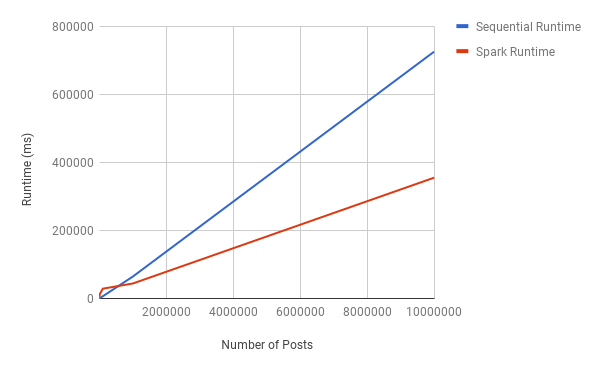
\includegraphics[width=\linewidth]{chart.png}
\end{figure}

Once more we observe that for our largest dataset of 10000000 posts, the Spark implementation was about slightly more than twice as fast as the sequential parser.  In addition, this dataset represents only a fraction of the total \so Data Dump, meaning the difference in execution times will be even larger when indexing the data dump in its entirety.

\section{Conclusion}
In conclusion, we have examined the application of the Apache Spark framework through the use case of calculating information retrieval metrics on a large corpus of documents, in this case posts from the \so Data Dump.  We have observed that for small datasets, less than about 60000 posts, the runtime of the sequential approach is faster than utilizing Spark.  However, for larger datasets, the runtime can be reduced in half by utilizing Spark over the sequential approach.  This is most likely due to the ability of Spark to distribute and parallelize the task of processing each post.
	
The results of this study are promising, as they illustrate the benefits Spark can provide, given a task is sufficiently parallelizable.  However, they also illustrate that for Spark to provide any benefits, the input dataset must be large, such that the overhead of distributing the task to multiple nodes in the cluster is outweighed by the runtime of the sequential implementation.    

Future research may focus on further optimizing the Spark implementation to reduce runtimes as well as introducing more complex and computationally expensive information retrieval metrics to be calculated while indexing to produce more sophisticated models.

% conference papers do not normally have an appendix


% use section* for acknowledgment
\section*{Acknowledgment}
The authors would like to thank Dr. Alberto Cano for providing guidance in the development of the Apache Spark implementation and for providing access to the server cluster on which our experiments were run. 

% trigger a \newpage just before the given reference
% number - used to balance the columns on the last page
% adjust value as needed - may need to be readjusted if
% the document is modified later
%\IEEEtriggeratref{8}
% The "triggered" command can be changed if desired:
%\IEEEtriggercmd{\enlargethispage{-5in}}

% references section

\bibliographystyle{IEEEtran}
\bibliography{stackintheflow}

% can use a bibliography generated by BibTeX as a .bbl file
% BibTeX documentation can be easily obtained at:
% http://mirror.ctan.org/biblio/bibtex/contrib/doc/
% The IEEEtran BibTeX style support page is at:
% http://www.michaelshell.org/tex/ieeetran/bibtex/
%\bibliographystyle{IEEEtran}
% argument is your BibTeX string definitions and bibliography database(s)
%\bibliography{IEEEabrv,../bib/paper}
%
% <OR> manually copy in the resultant .bbl file
% set second argument of \begin to the number of references
% (used to reserve space for the reference number labels box)

% that's all folks
\end{document}


